\documentclass{standalone}
\usepackage{tikz}
\usetikzlibrary{positioning,shapes.symbols}
%
\begin{document}

\begin{tikzpicture}
  \node[anchor=south west,inner sep=0] (image) at (0,0) {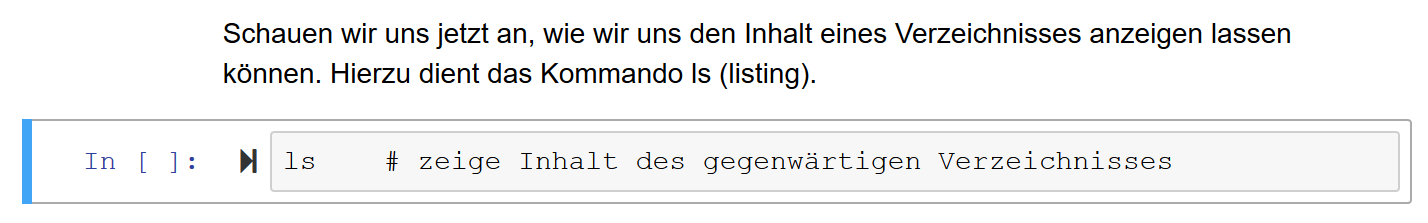
\includegraphics[width=5cm]{figuren/Text_Befehlszelle.png}};
  %
  \begin{scope}[x={(image.south east)},y={(image.north west)}]
    %\draw[help lines, ultra thin, step=0.02] (0,0) grid (1,1);
    %\draw[help lines, very thin,xstep=.1,ystep=.1] (0,0) grid (1,1);
    %\foreach \x in {0,1,...,9} { \node [font=\tiny, anchor=north] at (\x/10,0) {0.\x}; }
    %\foreach \y in {0,1,...,9} { \node [font=\tiny, anchor=east] at (0,\y/10) {0.\y}; }
    \node[fill = blue!10, font=\tiny, align = center] (befehl) at (0.5, -0.5) {Befehlszelle};
    \node[fill = red!10, font=\tiny, align = center] (text) at (0.5, 1.5) {Textzelle};
    \draw[red, thick] (0.08, 0.54) rectangle (0.96, 0.96);
    \draw[blue, thick] (0.007, 0.08) rectangle (0.99, 0.46);
    \draw[-latex, blue] (befehl) to (0.5, 0.08);
    \draw[-latex, red] (text) to (0.5, 0.96);
  \end{scope}
\end{tikzpicture}

\end{document}
